\documentclass[10pt,utf8]{beamer}

\mode<presentation> {
  \usetheme{Madrid}
  \setbeamercovered{transparent}
}

\usepackage{palatino}
\usepackage{graphicx}
\usepackage{array}
\usepackage{color}
\usepackage{subfigure}
\usepackage{colortbl}
\usepackage{amsmath}
\usepackage{hyperref}
\usepackage{listings}

\title{Improving the CI workflows with Docker}
\author[Vojtěch Juránek]{Vojtěch Juránek\newline\footnotesize{(\href{https://github.com/vjuranek}{\textcolor{blue}{https://github.com/vjuranek}}) }}
\institute[Red Hat]{JBoss - a division by Red Hat}
\date{7.~2.~2015, Developer conference, Brno}

\setbeamertemplate{caption}{\raggedright\insertcaption\par} %turn off caption prefix ("Figure")

\definecolor{darkGreen}{rgb}{0.3,0.7,0.3}
\definecolor{darkRed}{rgb}{0.7,0.3,0.3}

\newcommand*\proItem{\item[\color{darkGreen}\scalebox{0.9}{\LARGE{\textbf{+}}}]}
\newcommand*\conItem{\item[\color{darkRed}\scalebox{0.9}{\LARGE{\textbf{\textendash}}}]}


\newenvironment{mylisting}
{\begin{list}{}{\setlength{\leftmargin}{1em}}\item\scriptsize\bfseries}
{\end{list}}

\newenvironment{mytinylisting}
{\begin{list}{}{\setlength{\leftmargin}{1em}}\item\tiny\bfseries}
{\end{list}}


\begin{document}


\begin{frame}
 \titlepage
\end{frame}


\begin{frame}
  \frametitle{Outline}
  \begin{itemize}
    \item Ideas how to use containers for 
    \begin{itemize}
      \item minimizing false negatives during testing,
      \item making integration tests more easy,
      \item creating unified dev/QA/prod environment,
      \item etc.
    \end{itemize}
    \item Jenkins Docker plugins.
    \item Some other useful tools.
  \end{itemize}
\end{frame}


\begin{frame}
	\frametitle{Containers, Docker and all the other things}
	\begin{itemize}
		\item \href{https://www.youtube.com/watch?v=2KmNIoMMtWA\#t=190}{\beamergotobutton{Docker, Docker, Docker}} \dots a buzzword for $\sim$ 1.5 year.
		\pause
		\item So, is the Docker a silver bullet for CI/CD or testing?
		\pause
		\item Surprisingly \dots 
		\pause
		\item \dots no, it isn't :-)
		\pause
		\item \dots but still can help, at least little bit.
	\end{itemize}
\end{frame}

\begin{frame}
	\frametitle{Common CI issues}
	\begin{itemize}
		\item False negatives due to issues with build environment:
		\begin{itemize}
			\item missing or misconfigured tools,
			\item conflicting builds,
			\item some other kind of environment issue.
		\end{itemize}
		\item Unable to reproduce or debug a failure: 
		\begin{itemize}
			\item VM is already destroyed or returned back to the machine pool,
			\item another build already has done some changes, killed some processes etc.
		\end{itemize}
	\end{itemize}
\end{frame}
		
\begin{frame}
	\frametitle{Common CI issues}
	\begin{columns}
		\column{0.6\textwidth}
		\begin{itemize}
			\item Different dev, QA and prod environments. 
			\item Have you ever heard (or said:-) \textit{"It works on my machine just fine!"}?
			\begin{itemize}
				\item I did, many times, usually as \textit{"Jenkins is broken, because it fails tests which are passing on my machine!"}
			\end{itemize}
			\item In general, production environment is not easily available:
			\begin{itemize}
				\item can be pretty hard to implement in test suite,
				\item even setup itself can be quite time consuming.
			\end{itemize}
			\item Implement proper test environment or mock required services could be so expensive, that some integration test are not implemented at all.
			\item Speed! CI feedback has to be as quick as possible.
		\end{itemize}
		
		\column{0.35\textwidth}
		\begin{figure}
			\centering
			
\includegraphics[width=4cm]{./img/works_on_my_machine.eps}
			\caption{\tiny{Fig. from \href{http://blog.codinghorror.com/the-works-on-my-machine-certification-program/}{blog.codinghorror.com}}}
		\end{figure}
	\end{columns}
\end{frame}

\begin{frame}
	\frametitle{Tip \#1: Define and share your dev/prod environment}
	\begin{itemize}
		\item Unified environment for all involved teams as a container.
		\item Easy to do changes, no need to wait for admins to do the changes on your test servers.
		\item You can experiment and eventually share the changes in environment very easily.
		\item Other folks needn't to have knowledge how to setup all parts of your app properly and spend any time with configuration.
		\item If you hit any issue, you can easily share with others for investigation.
		\item There are of course other ways how to achieve it (tools like Puppet or distributing VMs), but Docker makes it super easy and fast.
		\item DevOps!
	\end{itemize}
\end{frame}

\begin{frame}
	\frametitle{Tip \#2: Use containers for build isolation}
	\begin{itemize}
		\item Run each build in fresh container.
		\item Very fast boot (c.f. to provisioning machine from Beaker of even to boot new machine in the cloud or VM).
		\item No interference with other builds or stale processes from previous build.
		\item Well defined environment for each build.
		\item Avoid "dependency hell" - OS has package ABC in version X, but my app needs it in version Y, while another needs it in version Z.
	\end{itemize}
\end{frame}

\begin{frame}
	\frametitle{Jenkins \& Docker}
	Sounds good? So, how to do it easily? \\ 
	Jenkins!
	\begin{figure}
		\centering
		
\includegraphics[width=5cm]{./img/jenkins_docker.eps}
	\end{figure}
	\begin{itemize}
		\item Jenkins CI has (AFAIK) the best Docker support in CI field - but still far from perfect.
		\begin{itemize}
			\item No blocker, but various minor, more or less annoying issues.
			\item Some useful features still missing.
		\end{itemize}
		\item However, other CI tools has limited or no Docker support at all.
	\end{itemize}
\end{frame}

\begin{frame}
	\frametitle{Jenkins Docker plugin \scriptsize{(\href{https://wiki.jenkins-ci.org/display/JENKINS/Docker+Plugin}{https://wiki.jenkins-ci.org/display/JENKINS/Docker+Plugin})}}
	\begin{itemize}
		\item ``Cloud'' provider of Docker slaves.
		\item Jenkins will dynamically start new containers and connect them as ordinary Jenkins slaves.
		\item Containers are created based on jobs waiting in the queue (according to labels assigned to jobs and containers).
		\item Once slaves are idle for some time, they are removed from Jenkins as well as from Docker.
		\vspace{0.5cm}
		\item Container has to have JVM and provide SSH service, you can use e.g.:
		\begin{itemize}
			\item Fedora slave: \texttt{docker pull vjuranek/jenkins-ssh-slave} \\
				\href{https://registry.hub.docker.com/u/vjuranek/jenkins-ssh-slave/}{\beamergotobutton{Docker Hub link}} 
			\item Ubuntu slave: \texttt{docker pull evarga/jenkins-slave} \\
				\href{https://registry.hub.docker.com/u/evarga/jenkins-slave/}{\beamergotobutton{Docker Hub link}}
		\end{itemize}
  \end{itemize}
\end{frame}

\begin{frame}
	\frametitle{Jenkins Docker plugin - configuration}
	Docker configuration:
	\begin{itemize}
		\item Docker server has to run with TCP port enabled:
		\item Add {{-H tcp://127.0.0.1:2375}} to Docker exec start options ({{/etc/systemd/system/docker.service}} on FC~20)
	\end{itemize}
	
	\begin{columns}
		\column{0.55\textwidth}
		Jenkins global configuration:
		\begin{itemize}
			\item Setup Docker URL.
			\vspace{0.5cm}
			\item Connection timeouts.
			\vspace{1cm}
			\item And maxim \# of containers which can run simultaneously.
		\end{itemize}
		
		\column{0.45\textwidth}
		\begin{figure}
			\centering
			\hspace{-1cm}
			
\includegraphics[width=5cm]{./img/docker_plugin_cfg1.eps}
		\end{figure}
	\end{columns}
\end{frame}

\begin{frame}
	\frametitle{Jenkins Docker plugin - configuration}
	\begin{columns}
		\column{0.55\textwidth}
		\begin{itemize}
			\item Assign labels to your images.
			\vspace{1cm}
			\item Setup SSH credentials
			\vspace{1cm}
			\item Configure the image (more in advanced settings).
			\vspace{1cm}
			\item Tight you jobs to required label.
		\end{itemize}
		
		\column{0.45\textwidth}
		\begin{figure}
			\centering
			\hspace{-1cm}
			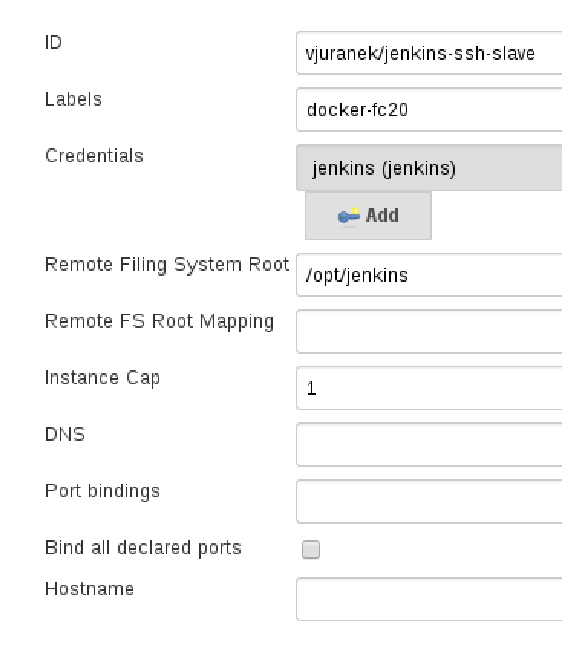
\includegraphics[width=6cm]{./img/docker_plugin_cfg2.eps}
		\end{figure}
	\end{columns}
\end{frame}


\begin{frame}[fragile]
  \frametitle{Create your custom container}
	Continue further with defining your own Jenkins slave image! \\
	\begin{itemize}
		\item Container needs to have JVM and Jenkins needs to be able to ssh to the container.
		\item Example Docker file based on Fedora:
	\end{itemize}

	\scriptsize{
		\begin{verbatim}
			FROM fedora:20                                                                                                                                                                                                   
MAINTAINER Vojtech Juranek <vjuranek@redhat.com>                                                                                                                                                                 
                                                                                                                                                                                                                 
# Execute system update                                                                                                                                                                                          
RUN yum -y update && yum clean all                                                                                                                                                                               
                                                                                                                                                                                                                 
# Install JDK and ssh server                                                                                                                                                                                     
RUN yum -y install java-1.7.0-openjdk-devel openssh-server && yum clean all                                                                                                                                      
                                                                                                                                                                                                                 
# Generate ssh key                                                                                                                                                                                               
RUN ssh-keygen -t rsa -f /etc/ssh/ssh_host_rsa_key -N ''                                                                                                                                                         
                                                                                                                                                                                                                 
# Create Jenkins user and Jenkins group                                                                                                                                                                          
RUN groupadd -r jenkins -g 1001 && useradd -u 1001 -r -g jenkins -m -d /opt/jenkins -s /bin/bash -c "Jenkins user" jenkins                                                                                       
RUN echo "jenkins:jenkins" | chpasswd                                                                                                                                                                            
                                                                                                                                                                                                                 
# Expose standard SSH port                                                                                                                                                                                       
EXPOSE 22                                                                                                                                                                                                        
                                                                                                                                                                                                                 
CMD ["/usr/sbin/sshd", "-D"]
		\end{verbatim}
	}
\end{frame}

\begin{frame}
	\frametitle{Jenkins Docker plugin}
	Per project configuration:
	\begin{columns}
	\column{0.55\textwidth}
		\begin{itemize}
			\item You can commit and push container when build succeeds.
			\item Start and stop containers during/after the build.
		\end{itemize}
		
	\column{0.55\textwidth}
	\begin{figure}
			\centering
			\hspace{-1cm}
			
\includegraphics[width=6cm]{./img/docker_plugin_cfg3.eps}
		\end{figure}
	\end{columns}
	
	\vspace{1cm}
	Pros and cons:
	\begin{itemize}
		\proItem Complex plug, which is able to handle a lot of things.
		\conItem Complex configuration.
		\conItem Sometimes not very easy to find out what could be wrong (especially when there is some bug in the plugin itself).
	\end{itemize}
\end{frame}

\begin{frame}
	\frametitle{Tip \#3: Embed you application into container}
	\begin{itemize}
		\item You can go one more step further and distribute you application embedded in the container.
		\begin{itemize}
			\item Not necessarily means that you have to deliver you app to customers as a container, you can use it just for testing.
		\end{itemize}
		\item Describe you build process in Docker file.
		\item Re-spins should be quite fast as Docker does \textbf{a lot of caching}.
		\item Sharing is very easy with Docker registry.
	\end{itemize}
	\begin{figure}
		\centering
		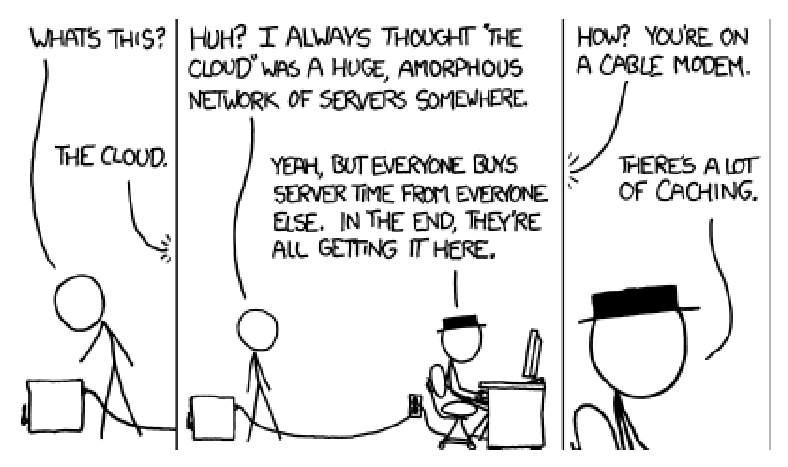
\includegraphics[width=7cm]{./img/xkcd_908.eps}
		\caption{\tiny{Part of \href{http://xkcd.com/908/}{xkcd \#908}}}
	\end{figure}
\end{frame}

\begin{frame}
	\frametitle{Jenkins Docker build publish plugin \scriptsize{(\href{https://wiki.jenkins-ci.org/display/JENKINS/Docker+build+publish+Plugin}{https://wiki.jenkins-ci.org/display/JENKINS/Docker+build+publish+Plugin})}}
	\begin{columns}
		\column{0.5\textwidth}
		\begin{figure}
			\centering
			\hspace{-1cm}
			
\includegraphics[width=4cm]{./img/All_You_Need_Is_Love.eps}
			\vspace{-0.5cm}
			\caption{\tiny{Source: \href{http://en.wikipedia.org/wiki/All_You_Need_Is_Love\#mediaviewer/File:All_You_Need_Is_Love_(Beatles_single_-_cover_art).jpg}{Wikipedia}}}
		\end{figure}
		
		\column{0.5\textwidth}
		\Large{\textbf{All you need is love ... and a Docker file!}}
	\end{columns}
	
	\begin{itemize}
		\item Plugin builds a Docker file and push the image into repository and registry.
		\item Useful especially for Docker-based applications.
		\item Useful mainly for private Docker registry, for public you can easily use Docker Hub automated builds to do the work for your.
		\begin{itemize}
			\item Could be e.g. the last step in dev build flow - project is built and Docker image is created.
			\item Create image can be subsequently consumed by QA, stage somewhere etc.
		\end{itemize}
	\end{itemize}
\end{frame}

\begin{frame}
	\frametitle{Tip \#4: Use Docker for better integration tests}
	\begin{itemize}
		\item Integration tests are sometimes pretty far from what happen in the production, as 
		\begin{itemize}
			\item there could be lots of simplifications, e.g. client/server apps communicate over loopback during the test,
			\item it's pretty hard to implement realistic scenarios,
			\item even setup itself can be quite time consuming.
		\end{itemize}
		\item Implement proper test environment or mocking of the services is so expensive, that some integration test are not implemented at all.
	\end{itemize}
	
	\vspace{0.7cm}
	
	\begin{itemize}
		\item With Docker, you can start real service during the integration test phase.
		\begin{itemize}
			\item Several ways how to achieve it.
			\item Start several services as Docker containers is pretty quick.
			\item Better than mocking or even running service from the test (e.g. network traffic is over vLANs etc.).
		\end{itemize}
		\item Testing is much more realistic and therefore valuable.
	\end{itemize}
\end{frame}

\begin{frame}
	\frametitle{Jenkins Docker build step plugin \scriptsize{(\href{https://wiki.jenkins-ci.org/display/JENKINS/Docker+build+step+plugin}{https://wiki.jenkins-ci.org/display/JENKINS/Docker+build+step+plugin})}}
	\begin{itemize}
		\item Allows you to add various Docker operation as a build step into your Jenkins project.
		\item Similar to Docker plugin you have to configure Docker URL in global Jenkins configuration.
		\begin{columns}
			\column{0.5\textwidth}
			\begin{itemize}
				\item Just select what you want to do in you project.
				\item Allows to wait for defined ports of started container to make sure container is fully running.
				\item Exports IP addresses as env. variables which can be consumed by other parts, etc.
			\end{itemize}
			\column{0.5\textwidth}
			\begin{figure}
				\centering
				
\includegraphics[width=5.5cm]{./img/docker-build-step-cfg1.eps}
			\end{figure}
		\end{columns}
		\item Unfortunately currently not compatible with Docker plugin.
	\end{itemize}
\end{frame}

\begin{frame}
	\frametitle{Some other useful Docker tools from the Java world}
	\begin{itemize}
		\item Jenkins is language agnostic, can be used with any kind of project.
		\item For various languages and frameworks exists dedicated tools.
		\item Not always you want Jenkins to be a central part of your processes.
		\item Sometimes you needs to run e.g. integration tests on you local machine and start Docker directly from your test suite or build tool.
		\item Examples of such tools from the Java world:
		\begin{itemize}
		 \item Maven Docker plugin(s)
		 \item Arquillian Cube
		\end{itemize}
	\end{itemize}
	
	\vspace{0.5cm}
	
	Not a Java developer?\\
	\begin{itemize}
		\item Never mind, there are tools also for other languages.
		\item Or implement Docker extension for your favorite framework.
		\item There are Docker client libraries for many languages, see \href{https://docs.docker.com/reference/api/remote_api_client_libraries/}{\textcolor{blue}{Docker Remote API Client Libraries}} list.
	\end{itemize}
\end{frame}

\begin{frame}
	\frametitle{Maven plugins for Docker}
	\begin{columns}
		\column{0.37\textwidth}
		\begin{itemize}
			\item There are many \textit{docker-maven} plugins.
			\item E.g. https://github.com/ alexec/docker-maven-plugin
		\end{itemize}
		
		\column{0.58\textwidth}
		\begin{figure}
			\centering
			\hspace{-1cm}
			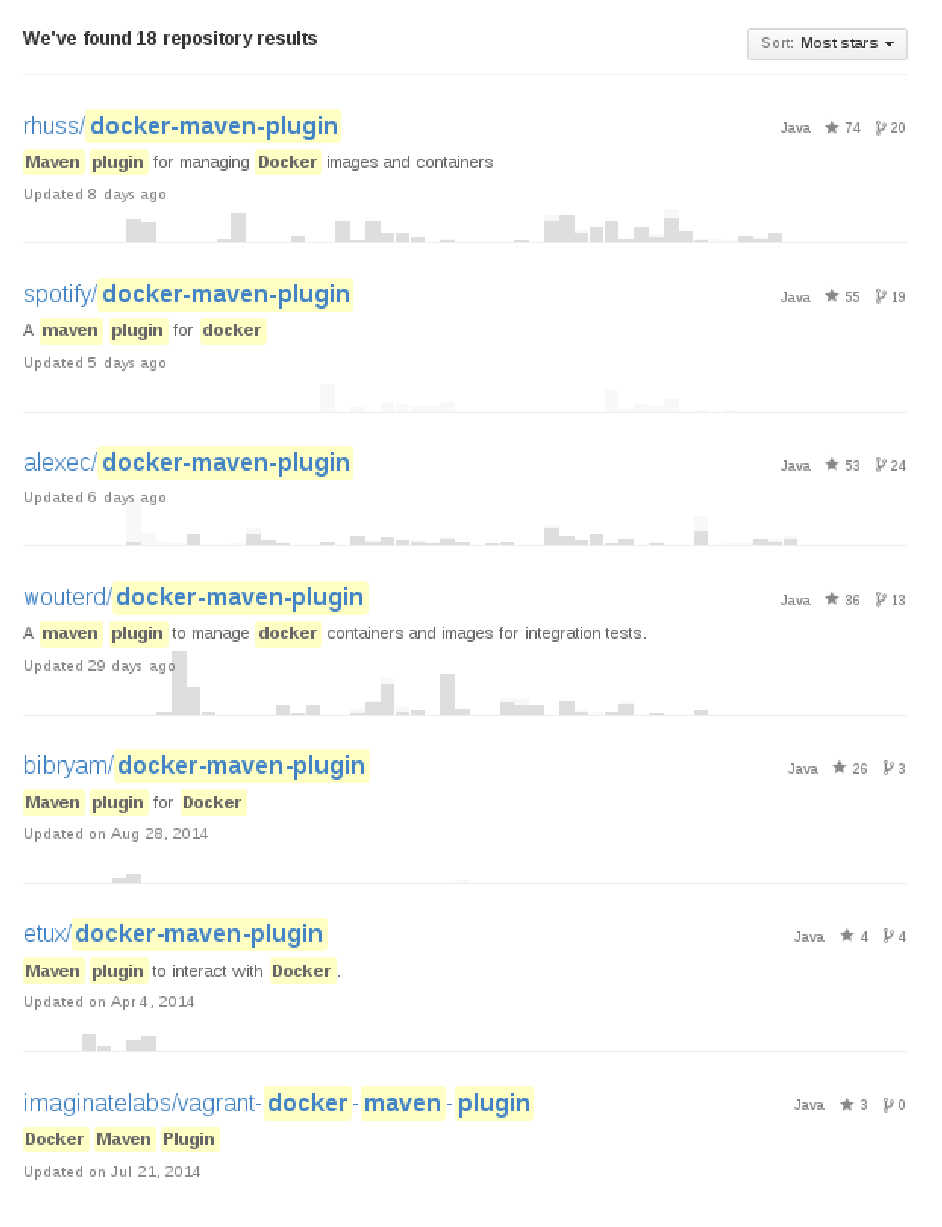
\includegraphics[width=7cm]{./img/docker-maven-plugin.eps}
		\end{figure}
	\end{columns}
\end{frame}

\begin{frame}[fragile]
  \frametitle{Docker Maven plugin}
	\begin{itemize}
		\item Place Docker file into \texttt{src/main/docker/your-app}
	\end{itemize}

	\scriptsize{
		\lstset{language=XML}
		\begin{lstlisting}
      [...]
      <plugin>
        <groupId>com.alexecollins.docker</groupId>
        <artifactId>docker-maven-plugin</artifactId>
        <configuration>
          <version>1.15</version>
          <host>http://127.0.0.1:2375</host>
        </configuration>
        <executions>
          <execution>
            <id>start-conatiner</id>
            <phase>pre-integration-test</phase>
            <goals>
              <goal>start</goal>
            </goals>
          </execution>
          [...]
        </executions>
      </plugin>
      [...]
		\end{lstlisting}
	}
\end{frame}

\begin{frame}[fragile]
	\frametitle{Integration with other tools}
	Maven Failsafe plugin:
		\scriptsize{
		\lstset{language=XML}
		\begin{lstlisting}
      [...]
      <plugin>
        <groupId>org.apache.maven.plugins</groupId>
        <artifactId>maven-failsafe-plugin</artifactId>
        <version>2.18.1</version>
        <configuration>
          <systemPropertyVariables>
            <demo.ldap.ip>${docker.ispn-ldap.ipAddress}</demo.ldap.ip>
          </systemPropertyVariables>
        </configuration>
        <executions>
          <execution>
            <goals>
              <goal>integration-test</goal>
              <goal>verify</goal>
            </goals>
          </execution>
        </executions>
      </plugin>
      [...]
		\end{lstlisting}
	}
\end{frame}

\begin{frame}[fragile]
	\frametitle{Arquillian Cube}
	\begin{itemize}
		\item Arquillian is a test runner with dependency injection, container life cycle management and other features.
		\item Arquillian Cube is Arquillian integration with Docker.
		\item Currently \texttt{1.0.0.Alpha} - you can expect further development.
	\end{itemize}
	Container definition in dedicated file \texttt{arquillian.xml}:
	\scriptsize{
		\begin{verbatim}
    <extension qualifier="docker">
      <property name="serverVersion">1.15</property>
      <property name="serverUri">http://localhost:2375</property>
      <property name="dockerContainers">
          ldap:
            image: vjuranek/docker-maven-demo_ispn-ldap
            exposedPorts: [389/tcp]
            await:
              strategy: polling
              sleepPollingTime: 2 s
      </property>
    </extension>

    <container qualifier="containerless" default="true">
      <configuration>
        <property name="containerlessDocker">ldap</property>
        <property name="embeddedPort">389</property>
      </configuration>
    </container>
		\end{verbatim}
	}
\end{frame}

\begin{frame}
	\frametitle{Demo}
	\begin{itemize}
		\item Trivial app which queries LDAP.
		\item LDAP server launched in the container.
		\item Available on \href{https://github.com/vjuranek/presentations/tree/master/DevConf_Brno2015/demo/docker-maven-demo}{\beamergotobutton{GitHub}}.
	\end{itemize}
	
	\vspace{0.5cm}
	
	\begin{itemize}
		\item Jenkins Docker build step plugin.
		\item Docker Maven plugin.
	\end{itemize}
	
	\vspace{0.5cm}
	
	\begin{itemize}
		\item Arquillian Cube, if some time remains.
	\end{itemize}
\end{frame}

\begin{frame}
	\frametitle{Putting it all together}
	\begin{itemize}
		\item Define you dev/prod environment in a Dockerfile and share the container(s) the other teams/team members.
		\item Use it for defining CI slave which exactly fits your needs.
		\item Build you application as a container.
		\item Use is for integration test which are executed in realistic production environment built on top of other containers.
		\item Automate everything in your CI system.
	\end{itemize}
\end{frame}

\begin{frame}
	\centering
	\huge{\textbf{Thank you for your attention!}} \\
	\vspace{1cm}
	\Large{\textbf{How do like it? Was it useful?}} \\
	\Large{\textbf{\href{http://devconf.cz/f/88}{Let me know on \textcolor{blue}{http://devconf.cz/f/88}}}}\\
	\vspace{1cm}
	\huge{\textbf{Questions?}}
\end{frame}


\end{document}